\documentclass{article}%
\usepackage[T1]{fontenc}%
\usepackage[utf8]{inputenc}%
\usepackage{lmodern}%
\usepackage{textcomp}%
\usepackage{lastpage}%
\usepackage[head=40pt,margin=0.5in,bottom=0.6in]{geometry}%
\usepackage{graphicx}%
%
\title{\textbf{Protesta en la Caracas{-}La Guaira mantiene bloqueada esta arteria vial}}%
\author{Diario El Universal}%
\date{19/09/2018}%
%
\begin{document}%
\normalsize%
\maketitle%
\textbf{URL: }%
http://www.eluniversal.com/caracas/21061/protesta{-}en{-}la{-}caracasla{-}guaira{-}mantiene{-}bloqueada{-}esta{-}arteria{-}vial\newline%
%
\textbf{Periodico: }%
EU, %
ID: %
21061, %
Seccion: %
caracas\newline%
%
\textbf{Palabras Claves: }%
NO\_TIENE\newline%
%
\textbf{Derecho: }%
2.8, %
Otros Derechos: %
, %
Sub Derechos: %
2.8.1\newline%
%
\textbf{EP: }%
SI\newline%
\newline%
%
\textbf{\textit{Los vecinos de los barrios El Limón, Tacagua Vieja y Nuevo Día decidieron cerrar la autopista en ambos sentidos desde hace más de una hora}}%
\newline%
\newline%
%
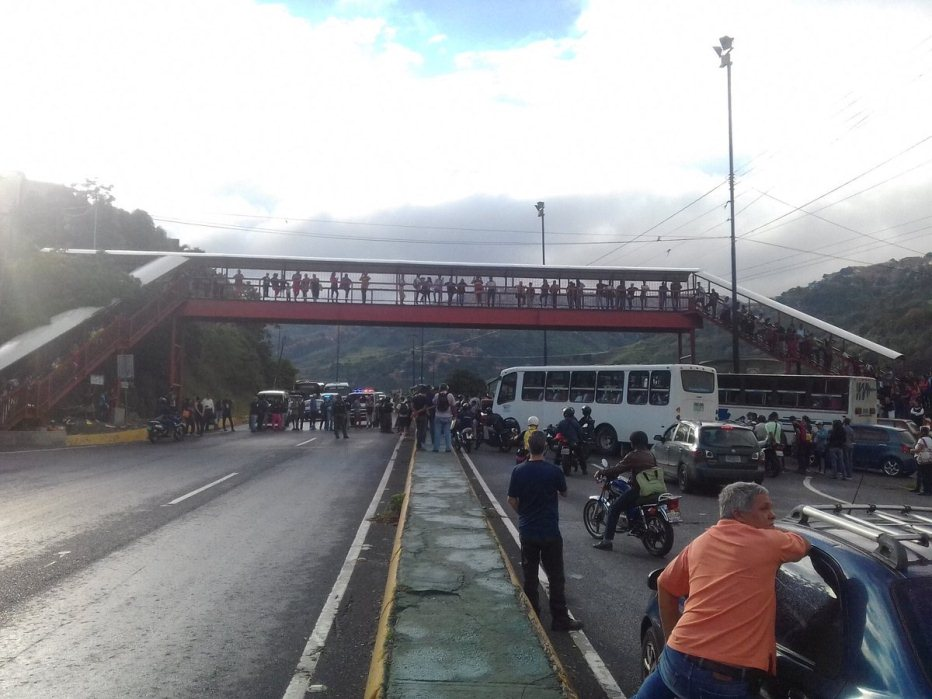
\includegraphics[width=300px]{69.jpg}%
\newline%
%
La autopista Caracas{-}La Guaira a la altura de El Limón permanece cerrada la mañana de este miércoles debido a una protesta por carencia de transporte público y fallas en el suministro de agua.%
\newline%
%
Los vecinos de los barrios El Limón, Tacagua Vieja y Nuevo Día decidieron cerrar la autopista en ambos sentidos desde hace más de una hora.%
\newline%
%
\end{document}